\documentclass[12pt]{article}
\usepackage{titling}
\usepackage[pdftex]{graphicx}
\usepackage[margin=1in]{geometry}
\linespread{1.3} %one-half spacing. 1.6 is double spaced. 
\frenchspacing
\usepackage{mathtools} %extra math symbols like arrows n shit
\usepackage[font=scriptsize]{caption}          %me being anal retentive about captions
\usepackage[raggedright]{sidecap}            %for side captions! Be aware, I don't think this is compatible with the float package...
		\sidecaptionvpos{figure}{c}        %centers captions vertically
\usepackage{gensymb}           %includes degree!
\usepackage{mhchem}        %There IS an easier way!
	%full isotope command: \ce{^{top#}_{bottom#}NameofElement^extraCrapAtTheEnd}  
	% ref: https://docs.moodle.org/27/en/Chemistry_notation_using_mhchem
\usepackage[font=scriptsize]{subcaption}  %because I just had to use a subcaption for one image. SIGH
\usepackage{simplewick}
\usepackage{amsmath}

\begin{document}


\section{Homework 1}

\subsection{Question 5}
$Q=M(\ce{^{223}_{88}Ra})-(M(\ce{^{14}_{6}C}+M(\ce{^{209}_{82}Pb})))=31.828$MeV

Then we can find the half-life from $T_{1/2}=\frac{\text{ln}2}{W P}$

with the decay rate defined as: 
 $W=\sqrt{\frac{Q}{2\mu R_t}}$ where $R_t$, the touching radius, is defined as $R_t=R_{decay product}+R_{daughter nucleus}$
 
 and the probability of decay defined as: 
 $P=$

Life tip: $e^2=1.44  \text{MeV}\cdot\text{fm}$


\newpage

\section{Project}
    
    \subsection{Part 1a}

Will type this later!

\subsection{Part 1b}
$H=H_0+H_1=
\begin{bmatrix}
	0 & 0\\
	0 & 2
	\end{bmatrix}
+
\begin{bmatrix}
	-g & -g \\
	-g & -g
	\end{bmatrix}
	=
\begin{bmatrix}
	-g & -g\\
	-g & 2-g\\
	\end{bmatrix}
	$
	\\
	\\
	Eigenvalues: 
	$1-g \pm \sqrt{g^2+1}$
	
	
\subsection{Part 1c: Hamiltonian Matrix}
No broken pairs, $S=0$, four lowest single particle levels filled by four particles. 

$H=H_0+H_1=\sum\limits_{p\sigma}  (p-1)a_{p\sigma}^\dagger a_{p\sigma} -g\sum\limits_{pq} P_{p}^{+}P_{q}^{-}$
\\
\\
$H_0=
\begin{bmatrix}
	2 & 0 & 0 & 0 & 0 & 0\\
	0 & 4 & 0 & 0 & 0 & 0 \\
	0 & 0 & 6 & 0 & 0 & 0\\
	0 & 0 & 0 & 6 & 0 & 0 \\
	0 & 0 & 0 & 0 & 8 & 0 \\
	0 & 0 & 0 & 0 & 0 & 10\\
\end{bmatrix}$
\\
\\
\\
$H_1=
\begin{bmatrix}
	-2g & -g & -g & -g & -g & 0\\
	-g & -2g & -g & -g & 0    & -g \\
	-g & -g & -2g & 0 & -g & -g\\
	-g & -g & 0 & -2g & -g & -g\\
	-g & 0 & -g & -g & -2g & -g\\
	0 & -g & -g & -g & -g & -2g\\
\end{bmatrix}$
\\
\\
\\
$H=H_0+H_1=
\begin{bmatrix}
	2-2g & -g & -g & -g & -g & 0\\
	-g & 4-2g & -g & -g & 0    & -g \\
	-g & -g & 6-2g & 0 & -g & -g\\
	-g & -g & 0 & 6-2g & -g & -g\\
	-g & 0 & -g & -g & 8-2g & -g\\
	0 & -g & -g & -g & -g & 10-2g\\
\end{bmatrix}$	



    
    
    
\newpage    
\section{Alex's email assignment from 7/7}
   Here's the interaction that goes with Gustav's talk today.

cceisdpn.int

You should use it with the sdpn.sp model space.

Before we meet at 2:30 your group should use this for our example of na23 and comment on

1) energy levels compared to exp

2) the extent to which isospin is conserved
    
    I put all this in the fridayex folder in rsh
    
\newpage




\section{NuShellX$^\copyright$ portion of project}



\subsection{A lot of neutron-rich isotope of Oxygen and Fluorine}

For USDB these agree quite well with the experimental results (when present) for a smaller sd-shell model. 



\subsection{$^{30}$F in the pf-shell: woo hoo!}

This uses the ``sdpf" model space and the ``sdpfu" interaction, which happened to be the first interaction on the list in that model space. 

Without extreme truncation, this is so computationally intense that NuShellX can't even calculate how long it would take to run the program. 

\newpage
 
$^{30}F$ in the pf-shell: closed neutron shell with one neutron in the fp-shell to move about
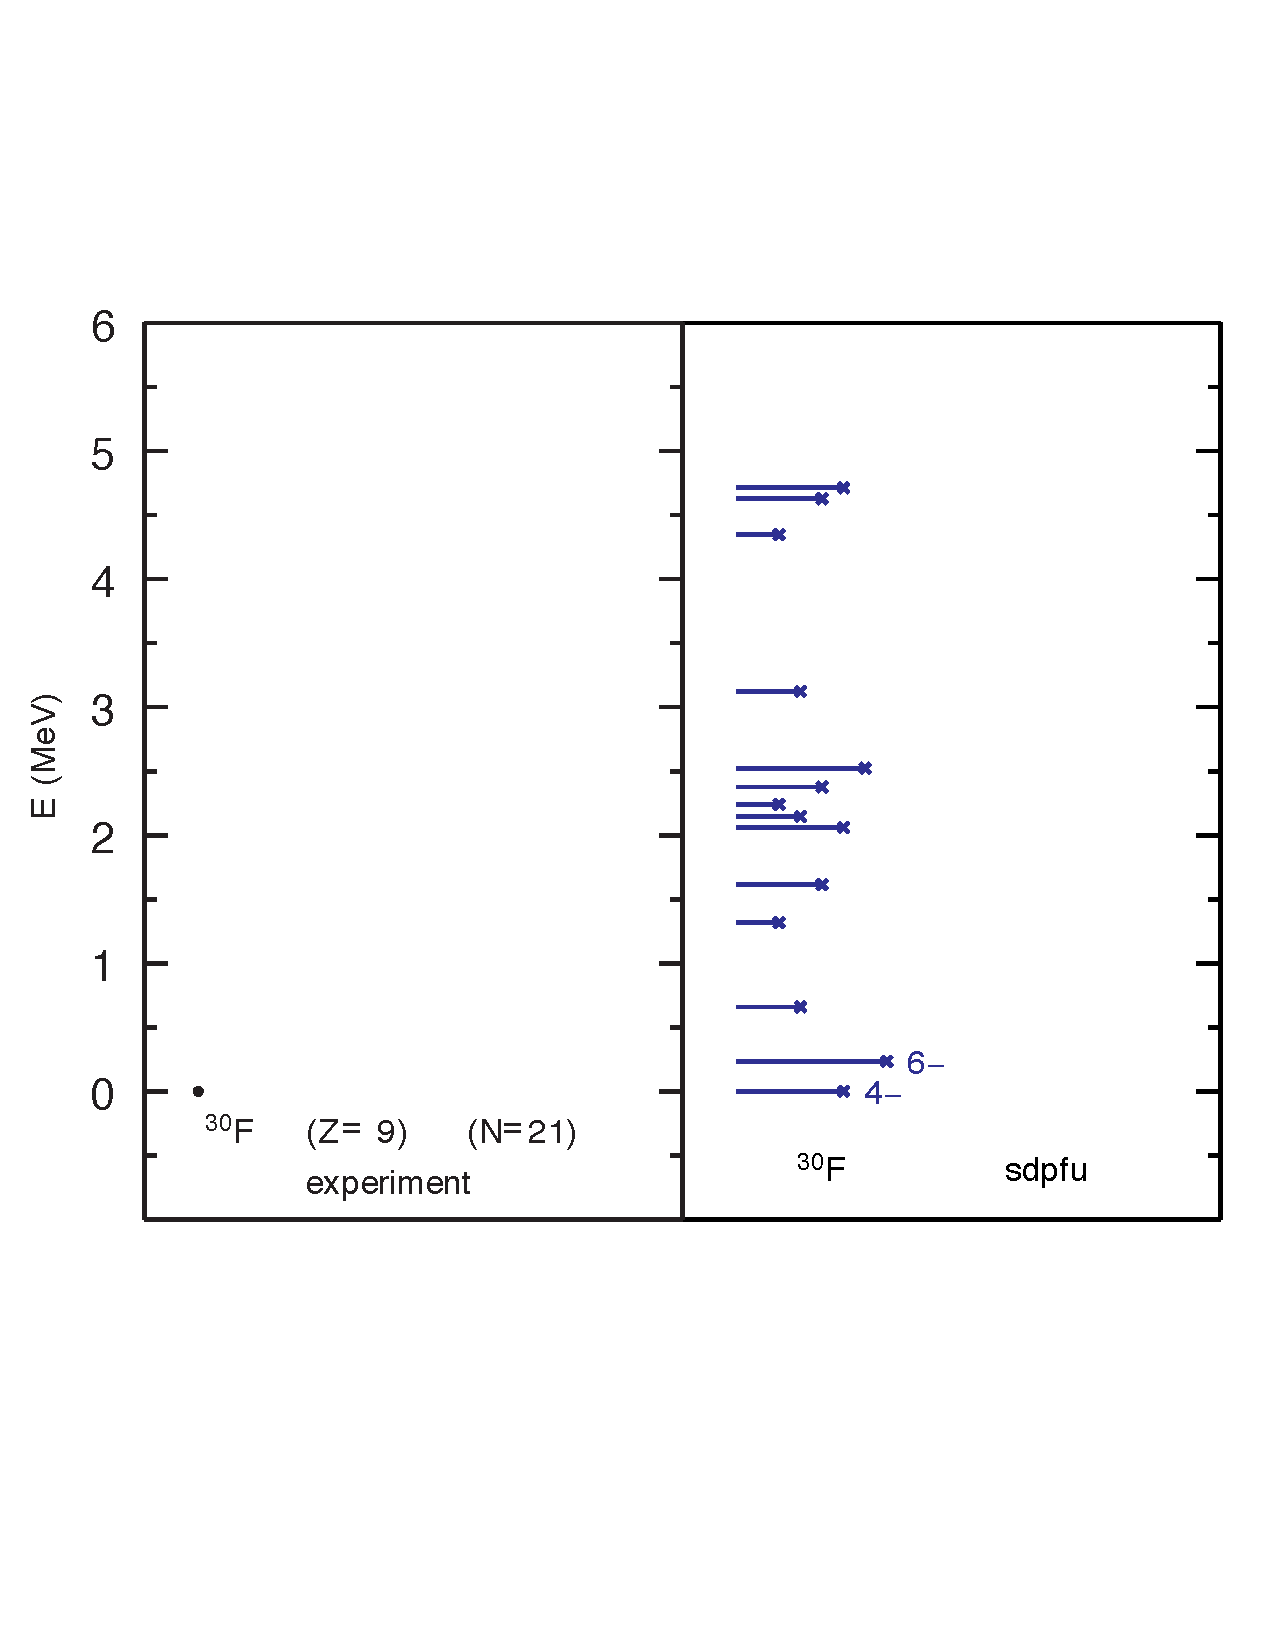
\includegraphics[width=\textwidth]{f_30u-1n.pdf}

\newpage

$^{30}$F in the pf-shell: 2 neutrons allowed in the fp-shell, 1 allowed out of the d3/2 shell

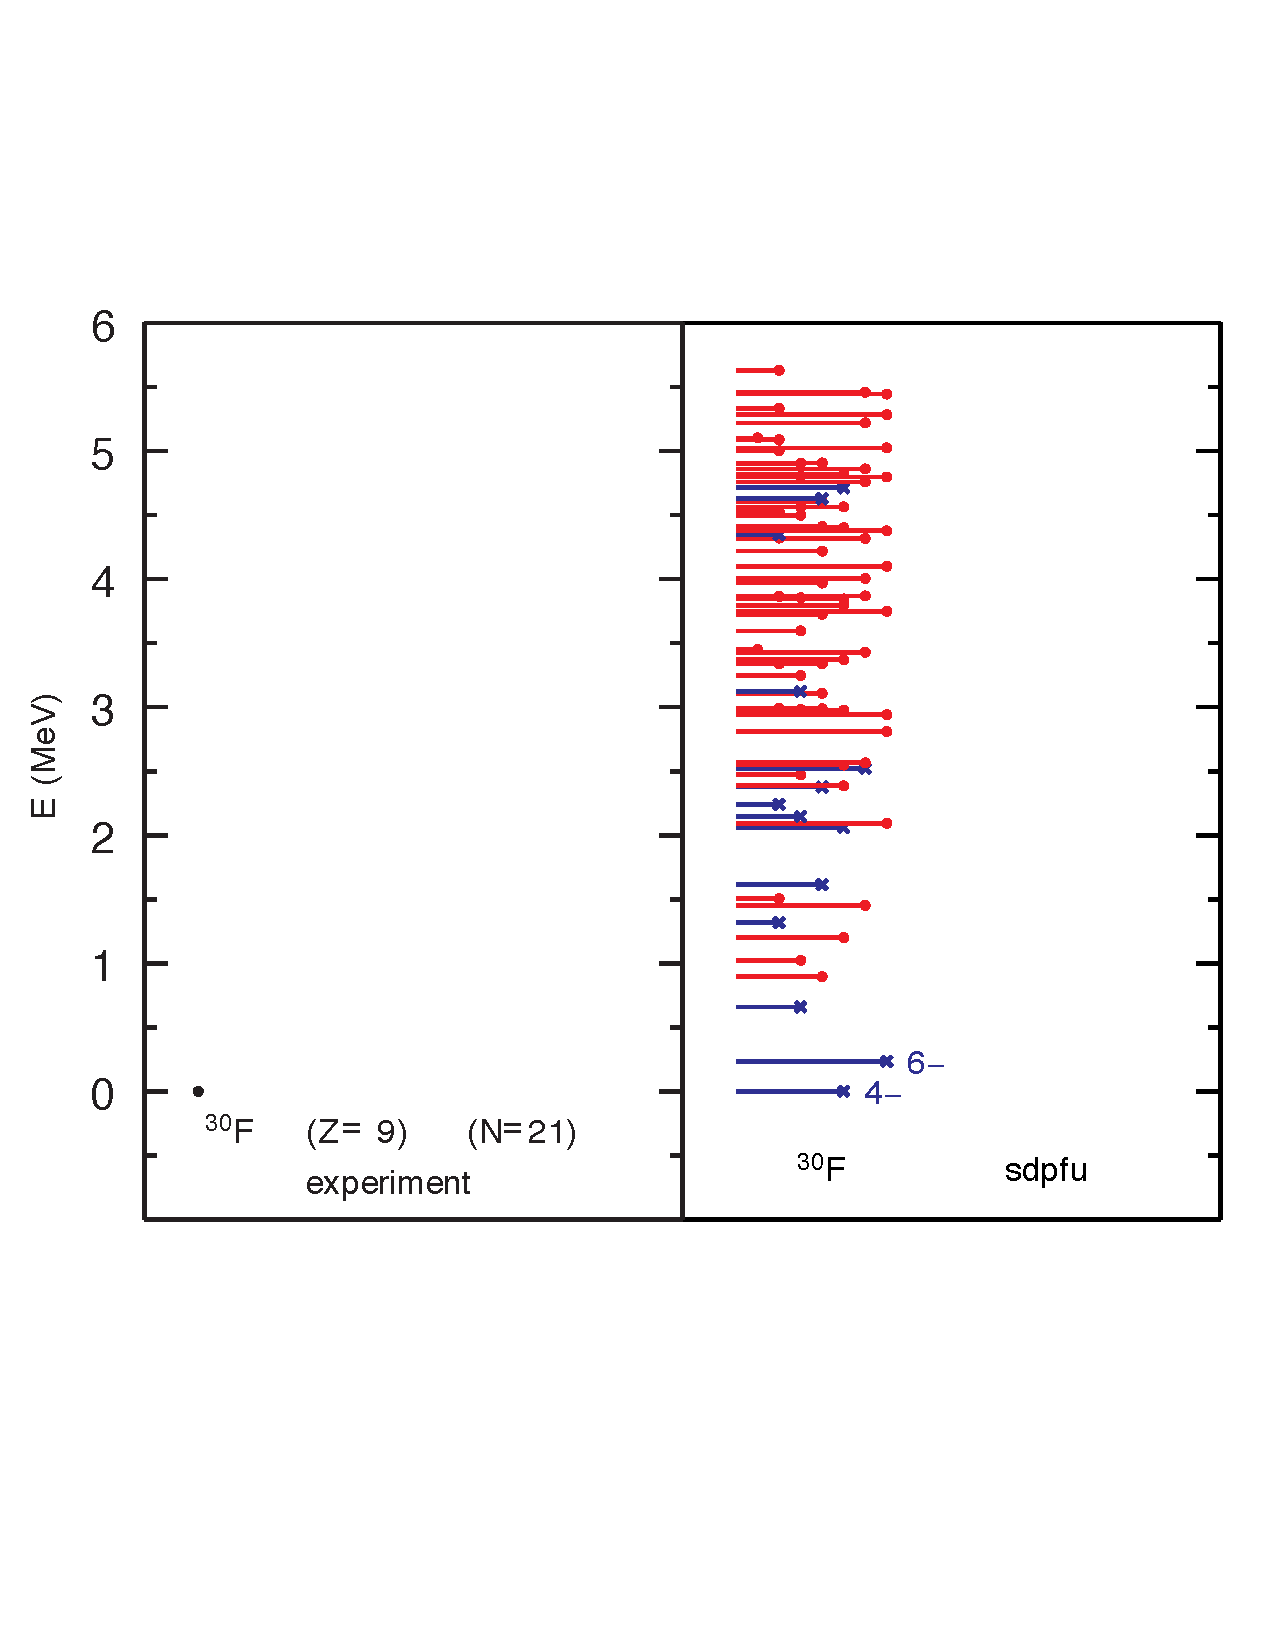
\includegraphics[width=\textwidth]{f_30u-2n.pdf} 
    
   \newpage
   
$^{30}$F in the pf-shell: 3 neutrons allowed in the fp-shell, 2 allowed out of the d3/2 shell

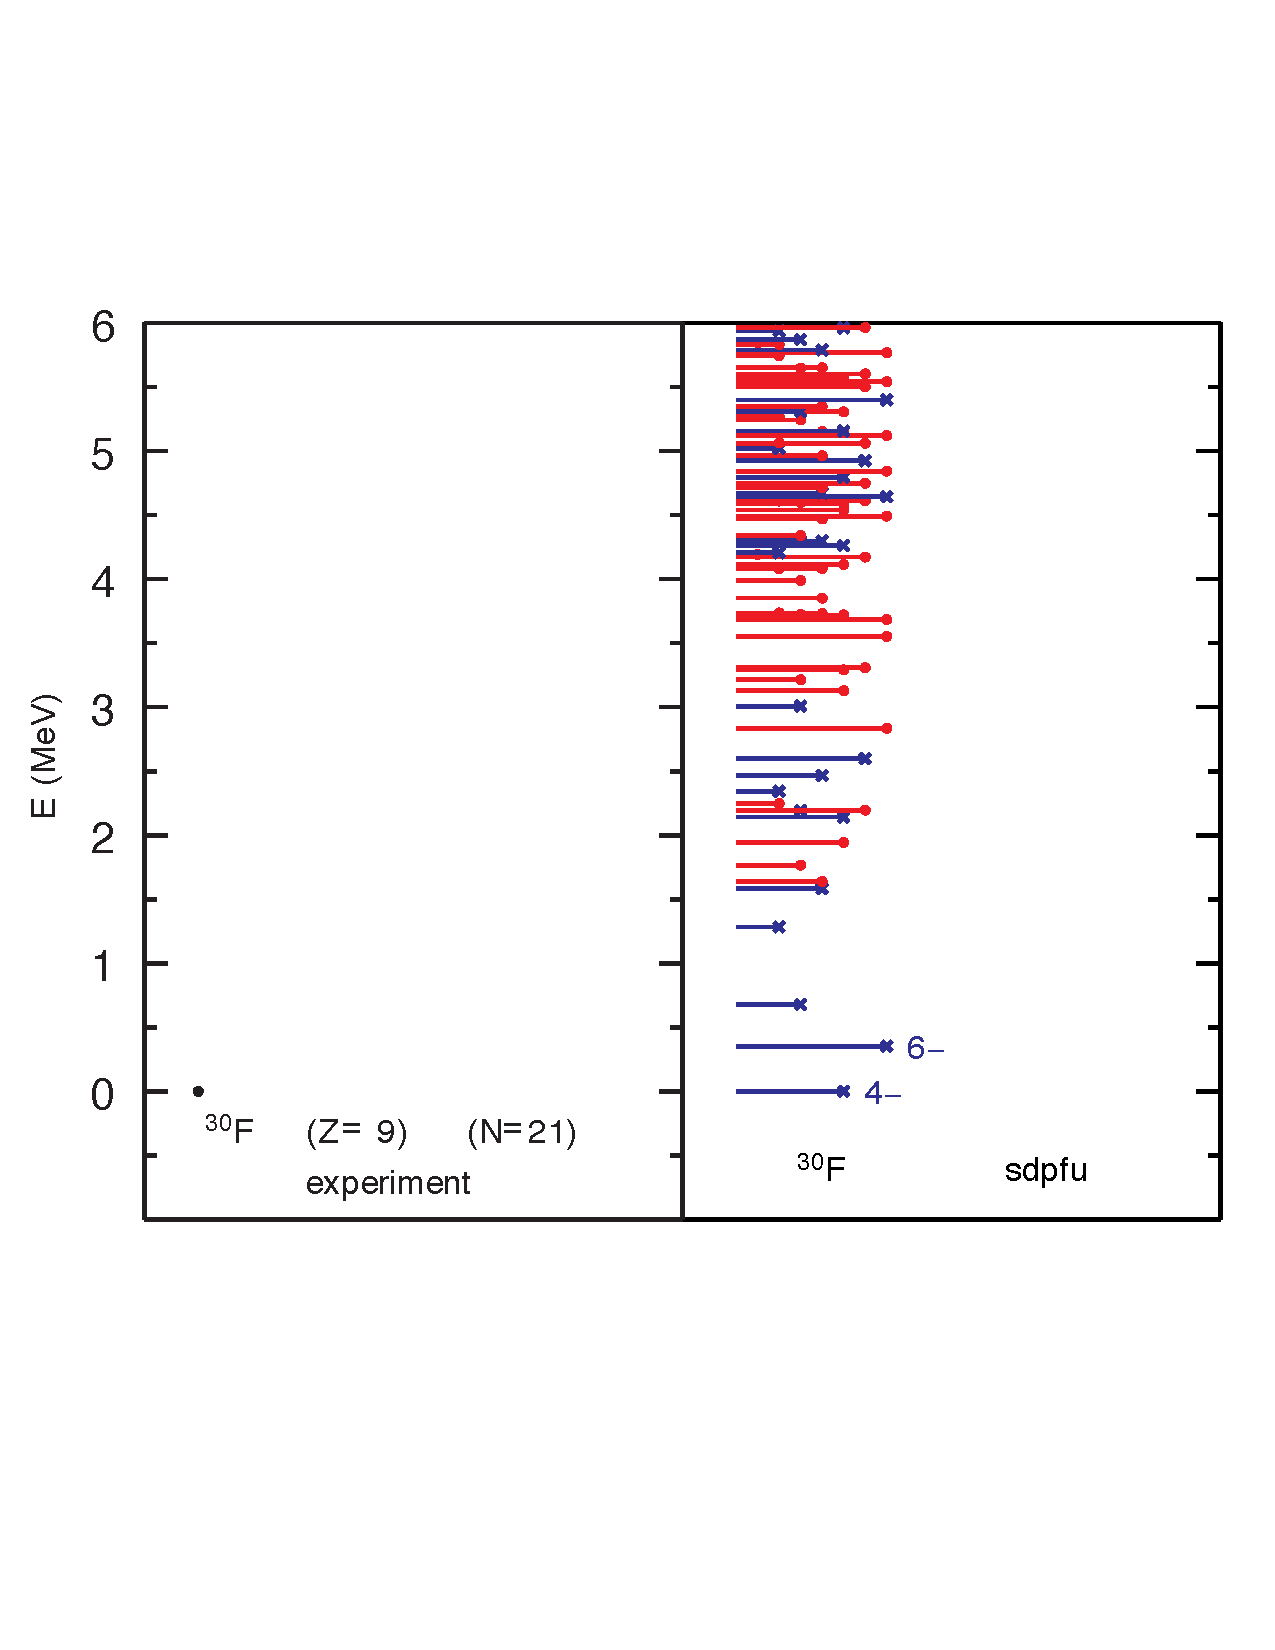
\includegraphics[width=\textwidth]{f_30u-3n.pdf}

\newpage

$^{30}$F in the pf-shell: all neutrons allowed out of the d3/2 shell into pf-shell

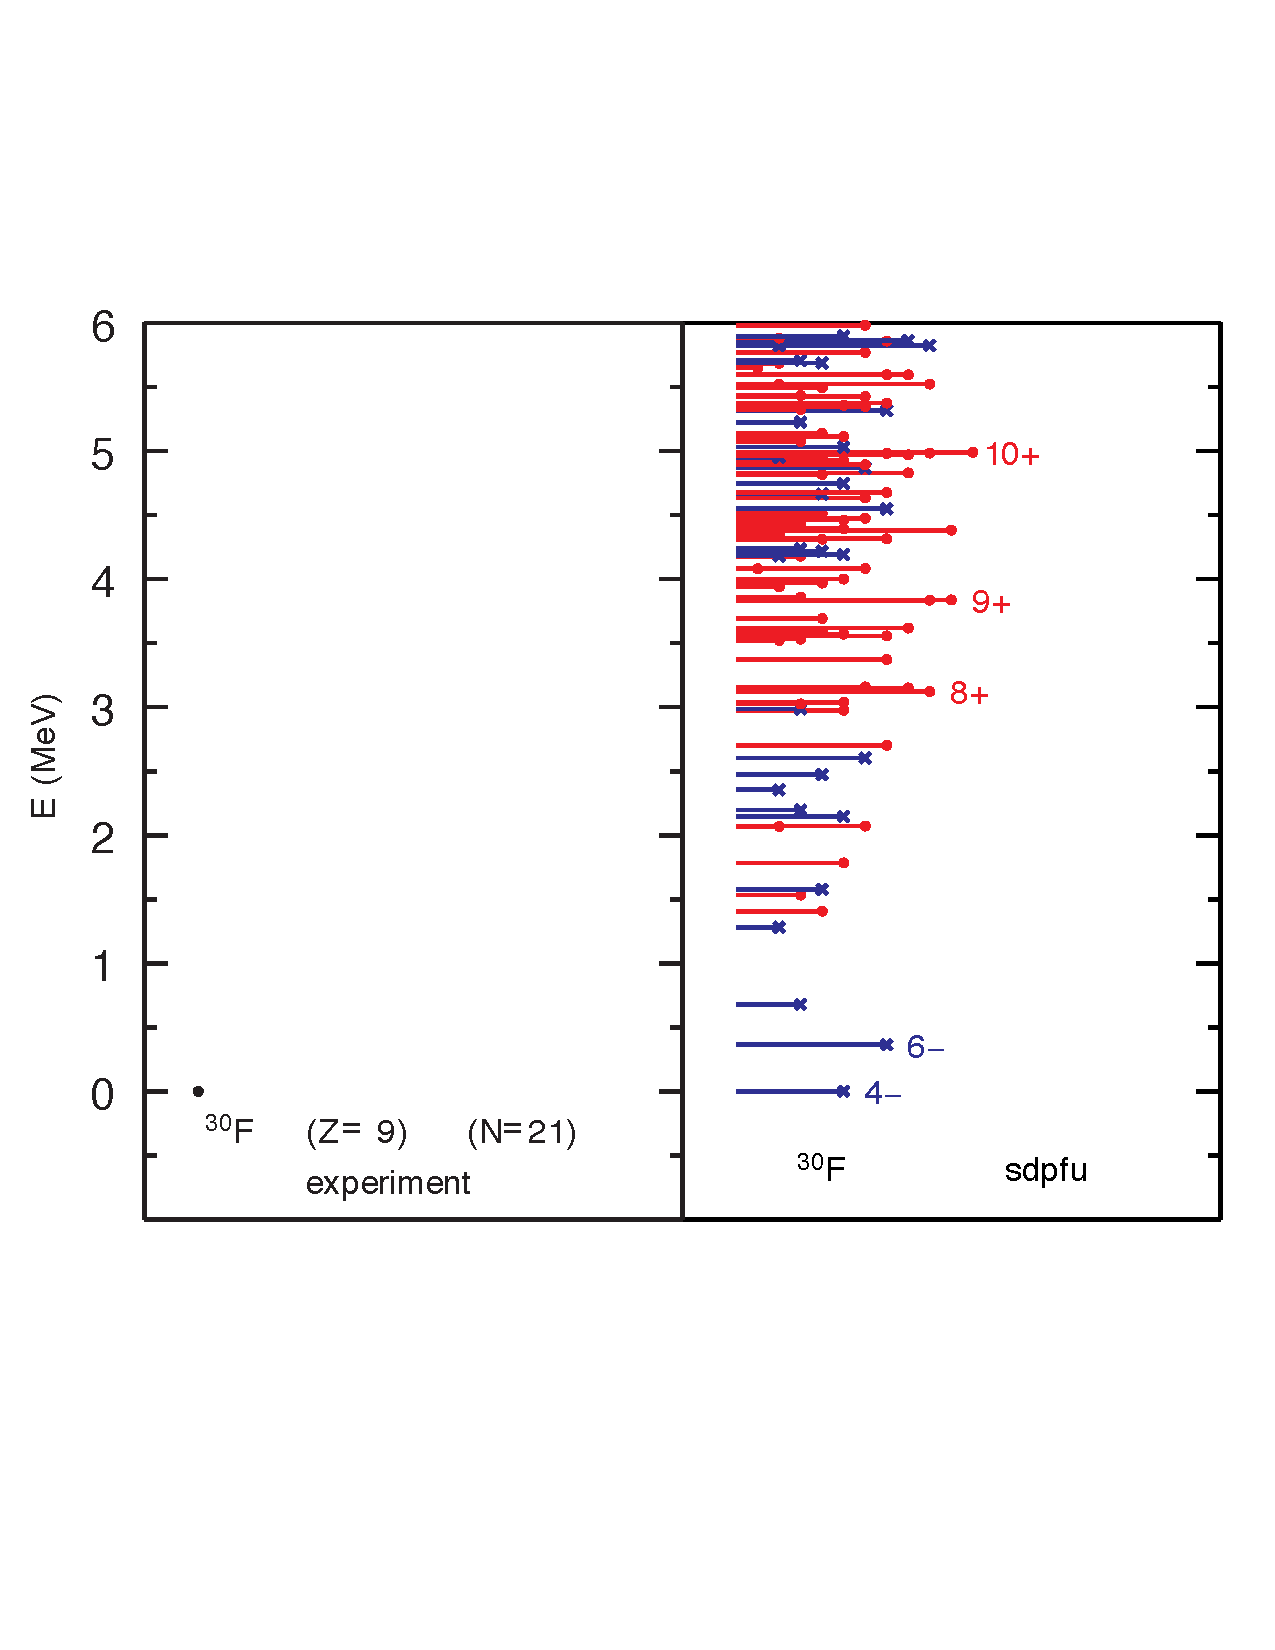
\includegraphics[width=\textwidth]{f_30u-allnfromd32.pdf}



\subsection{Some Spectroscopic Factors for Oxygen}

See specsb.lsf text file for results from \ce{^{23}O^{gnd}} to \ce{^{22}O^{any state}}


\end{document}